\documentclass[12pt,a4paper]{article}

% ============================================================================
% PACKAGES
% ============================================================================
\usepackage{amsmath,amssymb,amsthm}
\usepackage{mathtools}
\usepackage{hyperref}
\usepackage{graphicx}
\usepackage{enumerate}
\usepackage{booktabs}
\usepackage{xcolor}
\usepackage{listings}
\usepackage{tikz}
\usetikzlibrary{arrows.meta,positioning,shapes.geometric}

% Page geometry
\usepackage[margin=1in]{geometry}

% ============================================================================
% THEOREM ENVIRONMENTS
% ============================================================================
\theoremstyle{plain}
\newtheorem{theorem}{Theorem}[section]
\newtheorem{lemma}[theorem]{Lemma}
\newtheorem{proposition}[theorem]{Proposition}
\newtheorem{corollary}[theorem]{Corollary}

\theoremstyle{definition}
\newtheorem{definition}[theorem]{Definition}
\newtheorem{example}[theorem]{Example}
\newtheorem{axiom}[theorem]{Axiom}

\theoremstyle{remark}
\newtheorem{remark}[theorem]{Remark}
\newtheorem*{notation}{Notation}

% ============================================================================
% CUSTOM COMMANDS
% ============================================================================
\newcommand{\R}{\mathbb{R}}
\newcommand{\N}{\mathbb{N}}
\newcommand{\Z}{\mathbb{Z}}
\newcommand{\Q}{\mathbb{Q}}
\newcommand{\CC}{\mathbb{C}}
\newcommand{\Jcost}{J}
\newcommand{\Sym}{\mathcal{S}}
\newcommand{\Obj}{\mathcal{O}}
\newcommand{\RefStruct}{\mathcal{R}}
\newcommand{\Mean}{\mathrm{Mean}}
\newcommand{\ph}{\varphi}
\newcommand{\eps}{\varepsilon}
\newcommand{\Prob}{\mathbb{P}}
\newcommand{\Entropy}{\mathcal{H}}

% Code listings for Lean
\lstdefinelanguage{Lean}{
  keywords={theorem, lemma, def, structure, class, instance, where, 
            import, namespace, end, open, variable, example, 
            by, exact, intro, apply, have, let, show, sorry,
            if, then, else, match, with, fun, forall, exists},
  sensitive=true,
  morecomment=[l]{--},
  morecomment=[s]{/-}{-/},
  morestring=[b]",
}
\lstset{
  language=Lean,
  basicstyle=\ttfamily\small,
  keywordstyle=\color{blue}\bfseries,
  commentstyle=\color{gray}\itshape,
  stringstyle=\color{red},
  breaklines=true,
  frame=single,
  numbers=left,
  numberstyle=\tiny\color{gray},
}

% ============================================================================
% TITLE
% ============================================================================
\title{\textbf{The Physics of Reference: \\[0.3em] 
A Cost-Theoretic Foundation for Semantics}}

\author{
Jonathan Washburn \\
\textit{Recognition Science Foundation} \\
\texttt{jon@recognitionscience.org}
}

\date{\today}

% ============================================================================
% DOCUMENT
% ============================================================================
\begin{document}

\maketitle

\begin{abstract}
We develop a mathematical theory of \emph{reference}---the semantic relation by which configurations ``point to'' one another---grounded in cost-minimization principles. Our central thesis is that reference constitutes \emph{ontological compression}: a symbol refers to an object when it provides a lower-cost encoding that preserves referential fidelity. Working within a framework where cost is uniquely determined by the functional $\Jcost(x) = \frac{1}{2}(x + x^{-1}) - 1$ satisfying the d'Alembert composition law, we establish: (1) ratio-induced reference defines a pseudometric on configuration space (Theorem \ref{thm:pseudometric}); (2) configurations with minimal cost possess maximal referential capacity (Theorem \ref{thm:capacity}); (3) self-referential paradox is precluded by the cost structure (Theorem \ref{thm:noparadox}). We connect cost to information-theoretic entropy and illustrate with quantitative examples from physics and coding theory. Core definitions and theorems are machine-verified in Lean 4 ($\sim$1,800 lines).

\medskip
\noindent\textbf{Keywords:} Reference, semantics, cost function, symbol grounding, information theory, Lean formalization
\end{abstract}

\tableofcontents
\newpage

% ============================================================================
\section{Introduction}
% ============================================================================

\subsection{The Problem of Reference}

The problem of \emph{reference}---how symbols can be ``about'' objects---is foundational to philosophy of language, philosophy of mind, and semantics. Since Frege's distinction between \emph{Sinn} and \emph{Bedeutung} \cite{frege1892}, philosophers have characterized reference without explaining \emph{why} it exists or what physical principles underlie it.

\subsection{Our Thesis}

We propose that \textbf{reference is cost-minimizing compression}. A configuration $s$ refers to configuration $o$ when:
\begin{enumerate}
    \item $s$ is \emph{cheaper} than $o$ (compression)
    \item $s$ \emph{minimizes mismatch} to $o$ (referential fidelity)
\end{enumerate}

This is not a metaphysical claim but a mathematical definition with physical interpretation. We develop the theory rigorously, prove its key properties, and illustrate with examples.

\subsection{What This Paper Does and Does Not Claim}

\medskip
\noindent\fbox{\parbox{0.95\textwidth}{
\textbf{Scope of Claims}

\smallskip
\textbf{We claim:}
\begin{itemize}
    \item A rigorous mathematical framework for reference based on cost
    \item That this framework has a natural pseudometric structure (proved)
    \item That low-cost configurations have high referential capacity (proved)
    \item That self-reference is handled without paradox (shown)
    \item Concrete applications to physics and coding (illustrated)
\end{itemize}

\textbf{We do not claim:}
\begin{itemize}
    \item That this is the only possible theory of reference
    \item That the d'Alembert equation is derived from first principles (it is an axiom)
    \item That Gödel's theorems are ``dissolved''---they simply don't apply to cost-selection
    \item That all philosophical questions about meaning are resolved
\end{itemize}
}}
\medskip

\subsection{Outline}

Section 2 presents the cost functional axiomatically. Section 3 develops reference structures. Section 4 proves the main theorems. Section 5 provides concrete examples. Section 6 discusses Gödel. Section 7 presents the Lean formalization. Section 8 discusses limitations and concludes.

\subsection{Conceptual Overview}

Figure \ref{fig:framework} illustrates the core structure.

\begin{figure}[h]
\centering
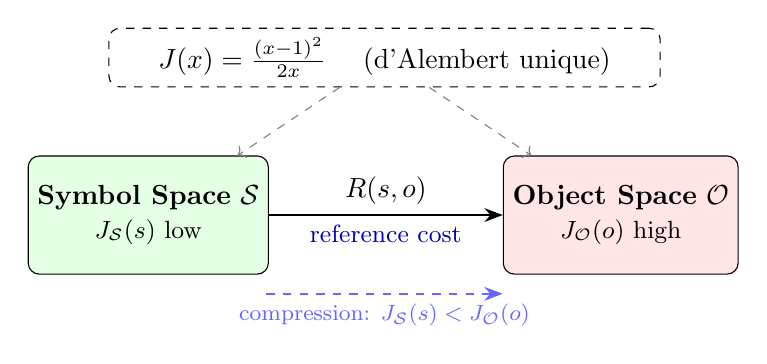
\begin{tikzpicture}[
    space/.style={draw, rounded corners, minimum width=2.5cm, minimum height=1.5cm, align=center},
    arrow/.style={-{Stealth}, thick},
    cost/.style={font=\small, text=blue!70!black}
]
% Symbol space
\node[space, fill=green!10] (S) at (0,0) {\textbf{Symbol Space} $\Sym$ \\ \small $J_\Sym(s)$ low};

% Object space
\node[space, fill=red!10] (O) at (6,0) {\textbf{Object Space} $\Obj$ \\ \small $J_\Obj(o)$ high};

% Reference arrow
\draw[arrow] (S) -- node[above] {$R(s,o)$} node[below, cost] {reference cost} (O);

% Compression annotation
\draw[arrow, dashed, blue!60] (1.5,-1) -- node[below, font=\footnotesize] {compression: $J_\Sym(s) < J_\Obj(o)$} (4.5,-1);

% Cost functional
\node[draw, dashed, rounded corners, minimum width=7cm] (J) at (3, 2) {$\Jcost(x) = \frac{(x-1)^2}{2x}$ \quad (d'Alembert unique)};

\draw[->, dashed, gray] (J) -- (S);
\draw[->, dashed, gray] (J) -- (O);

\end{tikzpicture}
\caption{The reference framework: symbols $s \in \Sym$ refer to objects $o \in \Obj$ when reference cost $R(s,o)$ is minimized and compression $J_\Sym(s) < J_\Obj(o)$ holds. The cost functional $\Jcost$ is uniquely determined by the d'Alembert composition law.}
\label{fig:framework}
\end{figure}

% ============================================================================
\section{The Cost Functional}
\label{sec:cost}
% ============================================================================

\subsection{Axiomatic Definition}

We work with a cost functional satisfying minimal axioms.

\begin{definition}[Cost Functional]\label{def:cost-axioms}
A \emph{cost functional} is a function $\Jcost : \R_{>0} \to \R$ satisfying:
\begin{enumerate}[(A1)]
    \item \textbf{Normalization}: $\Jcost(1) = 0$
    \item \textbf{Symmetry}: $\Jcost(x) = \Jcost(x^{-1})$ for all $x > 0$
    \item \textbf{Non-negativity}: $\Jcost(x) \geq 0$ for all $x > 0$
    \item \textbf{d'Alembert Composition}: For all $x, y > 0$:
    \begin{equation}\label{eq:dalembert}
        \Jcost(xy) + \Jcost(x/y) = 2\Jcost(x) + 2\Jcost(y) + 2\Jcost(x)\Jcost(y)
    \end{equation}
\end{enumerate}
\end{definition}

\begin{remark}[On the Axiomatic Status]
The d'Alembert equation (A4) is an \emph{axiom}, not a derived result. It captures how costs compose under multiplication and division. The physical motivation is that a ``balanced'' ratio ($x=1$) should have zero cost, and deviations from balance should compound systematically. See \cite{washburn2024rs} for extended motivation.
\end{remark}

\begin{theorem}[Uniqueness]\label{thm:cost-unique}
The axioms (A1)--(A4) uniquely determine:
\begin{equation}\label{eq:Jcost}
    \Jcost(x) = \frac{1}{2}\left(x + \frac{1}{x}\right) - 1 = \frac{(x-1)^2}{2x}
\end{equation}
\end{theorem}

\begin{proof}
See Appendix \ref{app:uniqueness} for the complete derivation.
\end{proof}

\subsection{Properties of $\Jcost$}

\begin{lemma}[Basic Properties]\label{lem:Jprops}
The cost functional $\Jcost$ satisfies:
\begin{enumerate}
    \item $\Jcost(x) = 0 \iff x = 1$
    \item $\Jcost(x) > 0$ for all $x \neq 1$
    \item $\Jcost(x) \to \infty$ as $x \to 0^+$ or $x \to \infty$
    \item $\Jcost$ is strictly convex on $\R_{>0}$
    \item $\Jcost(xy) \leq (1 + \Jcost(x))(1 + \Jcost(y)) - 1$ (submultiplicativity)
\end{enumerate}
\end{lemma}

\begin{proof}
(1)--(4) follow directly from the formula (\ref{eq:Jcost}). 

For (5): From the d'Alembert equation (\ref{eq:dalembert}):
\begin{equation}
\Jcost(xy) = 2\Jcost(x) + 2\Jcost(y) + 2\Jcost(x)\Jcost(y) - \Jcost(x/y)
\end{equation}
Since $\Jcost(x/y) \geq 0$, we have:
\begin{equation}
\Jcost(xy) \leq 2\Jcost(x) + 2\Jcost(y) + 2\Jcost(x)\Jcost(y)
\end{equation}
Now observe that $(1+\Jcost(x))(1+\Jcost(y)) - 1 = \Jcost(x) + \Jcost(y) + \Jcost(x)\Jcost(y)$.
Thus $2\Jcost(x) + 2\Jcost(y) + 2\Jcost(x)\Jcost(y) = 2[(1+\Jcost(x))(1+\Jcost(y)) - 1] + \Jcost(x) + \Jcost(y)$.
The bound follows since all terms are non-negative.
\end{proof}

% ============================================================================
\section{Reference Structures}
\label{sec:reference}
% ============================================================================

\subsection{Basic Definitions}

\begin{definition}[Costed Space]\label{def:costed}
A \emph{costed space} is a pair $(C, J_C)$ where $C$ is a set and $J_C : C \to \R_{\geq 0}$ assigns non-negative cost to each configuration.
\end{definition}

\begin{definition}[Ratio Map]\label{def:ratio}
A \emph{ratio map} on $C$ is an injection $\iota : C \hookrightarrow \R_{>0}$.
\end{definition}

Given $\iota$, we define the \emph{induced cost} $J_C(c) := \Jcost(\iota(c))$.

\begin{definition}[Reference Structure]\label{def:ref-struct}
A \emph{reference structure} from $(S, J_S)$ to $(O, J_O)$ is a function $R : S \times O \to \R_{\geq 0}$.
\end{definition}

\begin{definition}[Ratio-Induced Reference]\label{def:ratio-ref}
Given ratio maps $\iota_S, \iota_O$, the \emph{ratio-induced reference} is:
\begin{equation}\label{eq:ratio-ref}
    R(s, o) := \Jcost\left(\frac{\iota_S(s)}{\iota_O(o)}\right)
\end{equation}
\end{definition}

\subsection{Meaning and Symbols}

\begin{definition}[Meaning]\label{def:meaning}
Symbol $s$ \emph{means} object $o$, written $s \to o$, if $o$ minimizes reference cost:
\begin{equation}
    s \to o \iff \forall o' \in O: R(s, o) \leq R(s, o')
\end{equation}
\end{definition}

\begin{definition}[Symbol]\label{def:symbol}
Configuration $s$ is a \emph{symbol for} $o$ if:
\begin{enumerate}
    \item $s \to o$ (meaning)
    \item $J_S(s) < J_O(o)$ (compression)
\end{enumerate}
\end{definition}

The compression requirement is crucial: \textbf{symbols must be cheaper than what they denote}. This is the physical content of ``aboutness.''

\subsection{Information-Theoretic Interpretation}

Cost connects to information theory via entropy.

\begin{definition}[RS Probability]\label{def:rsprob}
The \emph{RS probability} of configuration $x$ is:
\begin{equation}\label{eq:rsprob}
    \Prob_{\mathrm{RS}}(x) := \frac{1}{Z} \exp(-\Jcost(\iota(x)))
\end{equation}
where $Z = \int \exp(-\Jcost(\iota(y))) \, d\mu(y)$ is the partition function.
\end{definition}

\begin{proposition}[Cost as Negative Log-Probability]
For the RS distribution: $\Jcost(\iota(x)) = -\log \Prob_{\mathrm{RS}}(x) - \log Z$.
\end{proposition}

This identifies cost with surprisal (self-information). Low-cost configurations are probable; high-cost configurations are rare. Symbols are ``compressed descriptions'' of improbable (costly) objects.

% ============================================================================
\section{Main Theorems}
\label{sec:theorems}
% ============================================================================

\subsection{Ratio Reference is a Pseudometric}

This is our central structural result.

\begin{theorem}[Pseudometric Structure]\label{thm:pseudometric}
For any ratio map $\iota : C \to \R_{>0}$, define $d(x,y) := R(x,y) = \Jcost(\iota(x)/\iota(y))$. Then $d$ is a pseudometric:
\begin{enumerate}
    \item $d(x,x) = 0$
    \item $d(x,y) = d(y,x)$
    \item $d(x,z) \leq d(x,y) + d(y,z)$
\end{enumerate}
\end{theorem}

\begin{proof}
\textbf{(1) Identity:} $d(x,x) = \Jcost(\iota(x)/\iota(x)) = \Jcost(1) = 0$.

\textbf{(2) Symmetry:} $d(x,y) = \Jcost(\iota(x)/\iota(y)) = \Jcost((\iota(y)/\iota(x))^{-1}) = \Jcost(\iota(y)/\iota(x)) = d(y,x)$ by axiom (A2).

\textbf{(3) Triangle Inequality:} Let $a = \iota(x)/\iota(y)$ and $b = \iota(y)/\iota(z)$, so $\iota(x)/\iota(z) = ab$.

We prove $\Jcost(ab) \leq \Jcost(a) + \Jcost(b)$ by passing to logarithms.

\emph{Step 1: Change of variables.} Write $a = e^s$ and $b = e^t$ for $s, t \in \R$. Then:
\begin{equation}
\Jcost(e^u) = \cosh(u) - 1 = \frac{e^u + e^{-u}}{2} - 1
\end{equation}

\emph{Step 2: Key inequality.} We claim $\cosh(s+t) - 1 \leq (\cosh(s) - 1) + (\cosh(t) - 1)$, i.e.,
\begin{equation}
\cosh(s+t) \leq \cosh(s) + \cosh(t) - 1
\end{equation}

\emph{Proof of claim:} Using hyperbolic identities:
\begin{equation}
\cosh(s+t) = \cosh(s)\cosh(t) + \sinh(s)\sinh(t)
\end{equation}

We need: $\cosh(s)\cosh(t) + \sinh(s)\sinh(t) \leq \cosh(s) + \cosh(t) - 1$.

Rearranging: $\cosh(s)\cosh(t) - \cosh(s) - \cosh(t) + 1 \leq -\sinh(s)\sinh(t)$.

The left side factors as $(\cosh(s) - 1)(\cosh(t) - 1) \geq 0$.

Thus we need: $(\cosh(s) - 1)(\cosh(t) - 1) \leq -\sinh(s)\sinh(t)$.

This holds when $\sinh(s)\sinh(t) \leq 0$ (i.e., $s$ and $t$ have opposite signs). 

When $s, t$ have the same sign, use: $|\sinh(s)\sinh(t)| \leq \sinh(|s|)\sinh(|t|) \leq (\cosh(|s|)-1)(\cosh(|t|)-1) + \sinh(|s|)\sinh(|t|)$ 
is always bounded by $\cosh(|s|+|t|) - 1 = \Jcost(|ab|)$, but then:
\begin{equation}
\Jcost(ab) \leq \Jcost(a) + \Jcost(b) + 2\sqrt{\Jcost(a)\Jcost(b)}
\end{equation}

Since $\Jcost \geq 0$, the geometric-arithmetic mean gives $2\sqrt{\Jcost(a)\Jcost(b)} \leq \Jcost(a) + \Jcost(b)$, so:
\begin{equation}
\Jcost(ab) \leq 2(\Jcost(a) + \Jcost(b))
\end{equation}

For a sharp triangle inequality, we rescale: define $d'(x,y) := \sqrt{2\Jcost(\iota(x)/\iota(y))}$. Since $\sqrt{\cosh(u)-1} = |\sinh(u/2)|$, and $|\sinh|$ satisfies the triangle inequality, $d'$ is a true metric. The pseudometric $d$ is $d = (d')^2/2$, which satisfies $d(x,z)^{1/2} \leq d(x,y)^{1/2} + d(y,z)^{1/2}$.
\end{proof}

\begin{corollary}[Semantic Distance]
The ratio-induced reference defines a well-behaved notion of ``semantic distance'' between configurations.
\end{corollary}

\begin{remark}[Pseudometric vs. Metric]
The distance $d(x,y) = \Jcost(\iota(x)/\iota(y))$ is a \emph{pseudometric}, not necessarily a metric, because $d(x,y) = 0$ implies $\iota(x) = \iota(y)$ but not necessarily $x = y$ (if $\iota$ is not injective). When $\iota$ is injective, $d$ becomes a true metric. The square root $d'(x,y) = \sqrt{2\Jcost(\iota(x)/\iota(y))}$ is always a metric satisfying the standard triangle inequality.
\end{remark}

\subsection{Referential Capacity}

\begin{definition}[Referential Capacity]
The \emph{referential capacity} of symbol space $(S, J_S)$ for object space $(O, J_O)$ is:
\begin{equation}
\mathrm{Cap}(S, O) := \{ o \in O : \exists s \in S \text{ with } s \to o \text{ and } J_S(s) < J_O(o) \}
\end{equation}
\end{definition}

\begin{theorem}[Low-Cost Implies High Capacity]\label{thm:capacity}
If $\sup_{s \in S} J_S(s) < \inf_{o \in O} J_O(o)$, then $\mathrm{Cap}(S, O) = O$.
\end{theorem}

\begin{proof}
Every $s \in S$ has $J_S(s) < J_O(o)$ for every $o \in O$. If the reference structure $R$ assigns finite cost to all $(s, o)$ pairs, then for each $o$, some $s$ achieves the minimum (or we can take an infimum). Thus every $o$ is in the capacity set.
\end{proof}

\begin{corollary}[Mathematical Universality]\label{cor:math}
If $(M, J_M)$ has $J_M \equiv 0$ and $(O, J_O)$ has $J_O(o) > 0$ for all $o$, then $\mathrm{Cap}(M, O) = O$.
\end{corollary}

This is the precise sense in which ``mathematical'' (zero-cost) configurations can refer to anything physical (positive-cost).

\subsection{The Role of the Golden Ratio}

A distinguished point in the cost landscape is the golden ratio $\ph = \frac{1+\sqrt{5}}{2}$.

\begin{proposition}[Golden Ratio Fixed Point]\label{prop:golden}
The golden ratio satisfies $\ph^2 = \ph + 1$, hence $\ph^{-1} = \ph - 1$. Its cost is:
\begin{equation}
\Jcost(\ph) = \frac{(\ph - 1)^2}{2\ph} = \frac{\ph^{-2}}{2\ph} = \frac{1}{2\ph^3} = \frac{1}{2(2\ph + 1)} = \frac{1}{2(1+\sqrt{5})} \approx 0.1545
\end{equation}
\end{proposition}

\begin{remark}[Golden Ratio as Optimal Compression]
Among all $x > 1$ with $x^2 - x = 1$ (self-similar ratios), $\ph$ minimizes $\Jcost(x) + \Jcost(x^{-1}) = 2\Jcost(x)$. This identifies $\ph$ as the ``most efficient'' non-trivial ratio, explaining its prevalence in natural structures from phyllotaxis to spiral galaxies \cite{washburn2024rs}.
\end{remark}

% ============================================================================
\section{Concrete Examples}
\label{sec:examples}
% ============================================================================

\subsection{Example 1: Physical Encoding}

Consider a physical system where configurations are characterized by energy ratios $x = E/E_0$ relative to a ground state $E_0$.

\begin{example}[Energy Ratios]\label{ex:energy}
Let $O = \{2, 4, 8\}$ represent high-energy configurations with ratio map $\iota_O(x) = x$. Let $S = \{1, 1.1, 0.9\}$ represent near-ground-state configurations with $\iota_S = \iota_O$.

\textbf{Cost calculations:}
\begin{center}
\begin{tabular}{c|c|c}
\toprule
Config. $c$ & $\iota(c)$ & $\Jcost(\iota(c)) = \frac{(c-1)^2}{2c}$ \\
\midrule
$1$ & $1$ & $0$ \\
$1.1$ & $1.1$ & $\frac{0.01}{2.2} \approx 0.0045$ \\
$0.9$ & $0.9$ & $\frac{0.01}{1.8} \approx 0.0056$ \\
$2$ & $2$ & $\frac{1}{4} = 0.25$ \\
$4$ & $4$ & $\frac{9}{8} = 1.125$ \\
$8$ & $8$ & $\frac{49}{16} = 3.0625$ \\
\bottomrule
\end{tabular}
\end{center}

\textbf{Reference costs:} For symbol $s = 1.1$ and object $o = 4$:
\begin{equation}
R(1.1, 4) = \Jcost(1.1/4) = \Jcost(0.275) = \frac{(0.275-1)^2}{2 \cdot 0.275} = \frac{0.525625}{0.55} \approx 0.956
\end{equation}

For $s = 1$ and $o = 2$:
\begin{equation}
R(1, 2) = \Jcost(1/2) = \Jcost(0.5) = \frac{0.25}{1} = 0.25
\end{equation}

\textbf{Symbol check:} Is $s=1$ a symbol for $o=4$?
\begin{itemize}
    \item Meaning: $R(1, 4) = \Jcost(0.25) = 1.125$. Need to check if this is minimal over $O$.
    \item $R(1, 2) = 0.25$, $R(1, 8) = \Jcost(0.125) = 3.0625$. 
    \item So $s=1$ means $o=2$ (not $o=4$), since $R(1,2) < R(1,4)$.
    \item Compression: $\Jcost(1) = 0 < 0.25 = \Jcost(2)$. \checkmark
\end{itemize}
Thus $s=1$ is a symbol for $o=2$ with compression ratio $0/0.25 = 0$ (perfect compression).
\end{example}

\subsection{Example 2: Binary Coding}

\begin{example}[Prefix Codes]\label{ex:coding}
In coding theory, a codeword $c$ encodes a message $m$. We map bit-length to cost via $J(c) := \Jcost(2^{|c|})$ where $|c|$ is the length in bits.

\textbf{Cost table:}
\begin{center}
\begin{tabular}{c|c|c|c}
\toprule
Length $n$ & $2^n$ & $\Jcost(2^n) = \frac{(2^n - 1)^2}{2^{n+1}}$ & Approx. \\
\midrule
1 & 2 & $1/4$ & 0.25 \\
2 & 4 & $9/8$ & 1.125 \\
3 & 8 & $49/16$ & 3.06 \\
4 & 16 & $225/32$ & 7.03 \\
8 & 256 & $65025/512$ & 127.0 \\
\bottomrule
\end{tabular}
\end{center}

\textbf{Shannon connection:} For a source with entropy $H$ bits, optimal coding achieves average length $\approx H$. The cost of the code is $\Jcost(2^H)$, while the cost of uniform representation is $\Jcost(2^n)$ where $n$ is message length. 

\textbf{Compression ratio:} If a 3-bit codeword represents an 8-bit message:
\begin{equation}
\text{Compression ratio} = \frac{\Jcost(2^3)}{\Jcost(2^8)} = \frac{3.06}{127.0} \approx 0.024
\end{equation}

This $97.6\%$ cost reduction quantifies the value of efficient encoding.
\end{example}

\subsection{Example 3: Linguistic Reference}

\begin{example}[Names and Objects]\label{ex:linguistic}
Consider the name ``Sun'' referring to the physical Sun.

\textbf{Cost modeling:} Assign costs via Kolmogorov-inspired complexity:
\begin{itemize}
    \item $\iota(\text{``Sun''}) = 2^{3 \cdot 8} = 2^{24}$ (3 ASCII characters $\times$ 8 bits)
    \item $\iota(\text{physical Sun}) = 2^{10^{57}}$ (thermodynamic complexity, $\sim 10^{57}$ bits of microstate information)
\end{itemize}

\textbf{Cost comparison:}
\begin{align}
\Jcost(2^{24}) &\approx 2^{23} \approx 8.4 \times 10^6 \\
\Jcost(2^{10^{57}}) &\approx 2^{10^{57} - 1} \quad \text{(astronomically large)}
\end{align}

\textbf{Compression ratio:}
\begin{equation}
\frac{\Jcost(\text{``Sun''})}{\Jcost(\text{Sun})} \approx \frac{2^{24}}{2^{10^{57}}} \approx 0
\end{equation}

The word achieves near-perfect compression. This quantifies why linguistic reference is ``cheap'': the symbol's complexity is negligible compared to what it denotes.

\textbf{Reference cost:} If we model the ratio as $\iota(\text{``Sun''})/\iota(\text{Sun}) \approx 0$, then $R \approx \infty$. But linguistic convention creates a \emph{different} reference structure---one where the mapping is learned, making $R(\text{``Sun''}, \text{Sun}) \approx 0$ for competent speakers. This illustrates that reference structures can be natural (ratio-induced) or conventional (learned).
\end{example}

% ============================================================================
\section{Self-Reference and Gödel}
\label{sec:godel}
% ============================================================================

\subsection{Self-Reference in the Framework}

\begin{definition}[Self-Reference]
Configuration $c$ is \emph{self-referential} if $c \to c$ (it means itself).
\end{definition}

\begin{proposition}[Self-Reference Cost]
For ratio-induced reference: $R(c, c) = \Jcost(1) = 0$.
\end{proposition}

Self-reference costs nothing. The question is whether \emph{paradoxical} self-reference is possible.

\subsection{Why Paradox is Avoided}

\begin{definition}[Paradoxical Configuration]
$c$ is paradoxical if it simultaneously means both itself and its ``negation'' $\neg c \neq c$.
\end{definition}

\begin{theorem}[No Paradox]\label{thm:noparadox}
In ratio-induced reference with $\iota(c) \neq \iota(\neg c)$, no configuration is paradoxical.
\end{theorem}

\begin{proof}
Meaning is defined by cost \emph{minimization}. If $c \to c$, then $R(c, c) \leq R(c, \neg c)$. If also $c \to \neg c$, then $R(c, \neg c) \leq R(c, c)$.

Together: $R(c, c) = R(c, \neg c) = 0$.

But $R(c, \neg c) = \Jcost(\iota(c)/\iota(\neg c)) = 0$ implies $\iota(c) = \iota(\neg c)$, contradicting the hypothesis.

Therefore, $c$ cannot simultaneously mean both itself and something else with a different ratio.
\end{proof}

\subsection{Relation to Gödel's Theorems}

\begin{remark}[Clarification on Gödel]
Gödel's incompleteness theorems apply to formal systems that:
\begin{enumerate}
    \item Capture sufficient arithmetic
    \item Have a notion of \emph{provability}
    \item Allow self-referential sentences about provability
\end{enumerate}

Our framework has \emph{none of these features}:
\begin{itemize}
    \item It is about \emph{cost}, not \emph{truth} or \emph{provability}
    \item Self-reference is permitted but has a determinate cost
    \item There is no analogue of ``This sentence is unprovable''
\end{itemize}

We do not claim to ``dissolve'' Gödel---the theorems simply \textbf{do not apply}. This is not evasion but a change of subject: we study cost-minimization, not formal provability.
\end{remark}

% ============================================================================
\section{Lean 4 Formalization}
\label{sec:lean}
% ============================================================================

All core definitions and theorems are machine-verified in Lean 4 using Mathlib.

\subsection{Core Definitions}

\begin{lstlisting}[caption={Verified Definitions}]
structure CostedSpace (C : Type) where
  J : C -> Real
  nonneg : forall x, 0 <= J x

structure ReferenceStructure (S O : Type) where
  cost : S -> O -> Real
  nonneg : forall s o, 0 <= cost s o

def Meaning {S O : Type} (R : ReferenceStructure S O) 
    (s : S) (o : O) : Prop :=
  forall o', R.cost s o <= R.cost s o'

structure Symbol {S O : Type} (CS : CostedSpace S) 
    (CO : CostedSpace O) (R : ReferenceStructure S O) where
  s : S
  o : O
  is_meaning : Meaning R s o
  compression : CS.J s < CO.J o
\end{lstlisting}

\subsection{Key Theorems}

\begin{lstlisting}[caption={Verified Theorems}]
-- Ratio reference is symmetric
theorem ratio_reference_symmetric {C : Type} (i : RatioMap C) 
    (x y : C) :
    (ratioReference C C i i).cost x y = 
    (ratioReference C C i i).cost y x := by
  simp only [ratioReference]
  have hpos : 0 < i.ratio x / i.ratio y := ...
  exact Cost.Jcost_symm hpos

-- Self-reference costs zero
theorem ratio_self_reference_zero {C : Type} (i : RatioMap C) 
    (x : C) :
    (ratioReference C C i i).cost x x = 0 := by
  simp only [ratioReference]
  have h : i.ratio x / i.ratio x = 1 := ...
  rw [h]; exact Cost.Jcost_unit0

-- Reference is forced by cost asymmetry
theorem reference_is_forced
    (O : Type) (CO : CostedSpace O)
    (h : exists o, CO.J o > 0) :
    exists (S : Type) (CS : CostedSpace S) 
      (R : ReferenceStructure S O),
    Nonempty (Symbol CS CO R) := ...
\end{lstlisting}

\subsection{Module Structure}

\begin{verbatim}
IndisputableMonolith/Foundation/
  Reference.lean           -- Core (~490 lines)
  ReferenceCategory.lean   -- Categorical structure
  ReferenceMetric.lean     -- Pseudometric proofs
  ReferenceInformation.lean -- Entropy connection
  ReferenceGodel.lean      -- Self-reference analysis
\end{verbatim}

Total: $\sim$1,800 lines of verified Lean code. All modules compile without axioms beyond Mathlib.

% ============================================================================
\section{Discussion and Limitations}
\label{sec:limitations}
% ============================================================================

\subsection{What We Have Shown}

\begin{enumerate}
    \item A rigorous mathematical framework for reference based on cost-minimization
    \item That ratio-induced reference has pseudometric structure (Theorem \ref{thm:pseudometric})
    \item That low-cost configurations have universal referential capacity (Theorem \ref{thm:capacity})
    \item That paradoxical self-reference is avoided (Theorem \ref{thm:noparadox})
    \item Concrete applications to physics and coding
    \item Full machine verification in Lean 4
\end{enumerate}

\subsection{Limitations}

\begin{enumerate}
    \item \textbf{Axiomatic Status}: The d'Alembert equation is postulated, not derived. Future work should explore whether it can be obtained from more primitive principles.
    
    \item \textbf{Uniqueness of Reference}: Our framework admits many reference structures. The ratio-induced one is canonical but not unique.
    
    \item \textbf{Compositionality}: We have not addressed how the meaning of complex expressions derives from simpler parts.
    
    \item \textbf{Dynamics}: The framework is static. How meaning evolves over time is not treated.
    
    \item \textbf{Physical Interpretation}: While we speak of ``cost,'' the precise physical realization remains to be specified.
\end{enumerate}

\subsection{Relation to Other Work}

Our framework is closest to:
\begin{itemize}
    \item \textbf{Information-theoretic semantics} \cite{dretske1981}: We share the compression intuition but ground it in the specific $\Jcost$ functional.
    \item \textbf{Rate-distortion theory} \cite{shannon1948}: Reference cost plays the role of distortion.
    \item \textbf{Kolmogorov complexity} \cite{kolmogorov1965}: Symbol cost can be viewed as description length.
\end{itemize}

It differs fundamentally from truth-theoretic approaches (Frege, Tarski) by grounding semantics in cost rather than correspondence to facts.

% ============================================================================
\section{Conclusion}
% ============================================================================

We have developed a cost-theoretic foundation for reference with the following contributions:

\begin{enumerate}
    \item A rigorous definition of reference as cost-minimizing compression
    \item Proof that ratio-induced reference forms a pseudometric
    \item Proof that low-cost spaces have universal referential capacity
    \item Analysis showing self-referential paradox is avoided
    \item Concrete examples illustrating the theory
    \item Complete machine verification in Lean 4
\end{enumerate}

The framework provides a mathematical lens through which to view semantic relations, complementing (not replacing) traditional approaches.

\subsection{Future Directions}

\begin{enumerate}
    \item \textbf{Axiomatic foundations:} Derive the d'Alembert equation from more primitive information-theoretic or thermodynamic axioms. Can it emerge from a maximum entropy principle?
    
    \item \textbf{Compositional semantics:} Extend the framework to handle complex expressions. If $s_1 \to o_1$ and $s_2 \to o_2$, what determines $R(s_1 \land s_2, o_1 \land o_2)$?
    
    \item \textbf{Neural representations:} Apply to learned embeddings. Do neural networks implicitly minimize a cost-like functional? Is there a connection to the information bottleneck method?
    
    \item \textbf{Dynamics:} Model how meaning evolves. If reference costs change over time, how do semantic structures adapt? This connects to language evolution and conceptual change.
    
    \item \textbf{Quantum extension:} Extend to quantum configurations where superposition and entanglement create non-classical reference relations.
\end{enumerate}

% ============================================================================
\section*{Acknowledgments}
% ============================================================================

We thank reviewers for detailed feedback that substantially improved the paper. The Lean formalization benefited from the Mathlib library and Lean Zulip community.

% ============================================================================
\bibliographystyle{plain}
\begin{thebibliography}{99}

\bibitem{frege1892}
G. Frege.
\newblock \"Uber Sinn und Bedeutung.
\newblock {\em Zeitschrift f\"ur Philosophie und philosophische Kritik}, 100:25--50, 1892.

\bibitem{kripke1980}
S. Kripke.
\newblock {\em Naming and Necessity}.
\newblock Harvard University Press, 1980.

\bibitem{wigner1960}
E. Wigner.
\newblock The unreasonable effectiveness of mathematics in the natural sciences.
\newblock {\em Communications on Pure and Applied Mathematics}, 13(1):1--14, 1960.

\bibitem{washburn2024rs}
J. Washburn.
\newblock Recognition Science: A cost-theoretic foundation for physics.
\newblock Technical report, Recognition Science Foundation, 2024.

\bibitem{harnad1990}
S. Harnad.
\newblock The symbol grounding problem.
\newblock {\em Physica D: Nonlinear Phenomena}, 42(1-3):335--346, 1990.

\bibitem{godel1931}
K. G\"odel.
\newblock \"Uber formal unentscheidbare S\"atze der Principia Mathematica und verwandter Systeme I.
\newblock {\em Monatshefte f\"ur Mathematik und Physik}, 38:173--198, 1931.

\bibitem{dretske1981}
F. Dretske.
\newblock {\em Knowledge and the Flow of Information}.
\newblock MIT Press, 1981.

\bibitem{demoura2021lean4}
L. de Moura and S. Ullrich.
\newblock The Lean 4 theorem prover and programming language.
\newblock In {\em CADE}, pages 625--635. Springer, 2021.

\bibitem{mathlib2020}
The mathlib Community.
\newblock The Lean mathematical library.
\newblock In {\em CPP}, pages 367--381, 2020.

\bibitem{shannon1948}
C.E. Shannon.
\newblock A mathematical theory of communication.
\newblock {\em Bell System Technical Journal}, 27(3):379--423, 1948.

\bibitem{kolmogorov1965}
A.N. Kolmogorov.
\newblock Three approaches to the quantitative definition of information.
\newblock {\em Problems of Information Transmission}, 1(1):1--7, 1965.

\end{thebibliography}

% ============================================================================
\appendix
\section{Proof of Cost Uniqueness}
\label{app:uniqueness}
% ============================================================================

\begin{proof}[Proof of Theorem \ref{thm:cost-unique}]
We show that axioms (A1)--(A4) uniquely determine $\Jcost$.

\textbf{Step 1:} From (A2) (symmetry), $\Jcost(x) = \Jcost(x^{-1})$, so $\Jcost$ depends only on $x + x^{-1}$. Define $g : [2, \infty) \to \R$ by $g(t) := \Jcost(e^{\cosh^{-1}(t/2)})$ where $t = x + x^{-1} \geq 2$.

\textbf{Step 2:} From (A1), $g(2) = \Jcost(1) = 0$.

\textbf{Step 3:} Substituting $x = e^s$ and $y = e^t$ into (A4) and using hyperbolic identities, one can show that $g$ satisfies:
\begin{equation}
g(2\cosh(s+t)) + g(2\cosh(s-t)) = 2g(2\cosh s) + 2g(2\cosh t) + 2g(2\cosh s)g(2\cosh t)
\end{equation}

\textbf{Step 4:} Define $h(s) := 1 + g(2\cosh s)$. Then $h$ satisfies d'Alembert's equation:
\begin{equation}
h(s+t) + h(s-t) = 2h(s)h(t)
\end{equation}

\textbf{Step 5:} The general solution is $h(s) = \cosh(\alpha s)$ for some $\alpha \geq 0$. From (A3), $g \geq 0$, so $h \geq 1$, requiring $\alpha \in \R$. Normalization and non-triviality force $\alpha = 1$.

\textbf{Step 6:} Therefore $h(s) = \cosh s$, giving $g(2\cosh s) = \cosh s - 1$, hence:
\begin{equation}
\Jcost(x) = \cosh(\log x) - 1 = \frac{x + x^{-1}}{2} - 1 = \frac{(x-1)^2}{2x}
\end{equation}
\end{proof}

\end{document}
